\begin{figure}[t]
  \centering
  \resizebox {\columnwidth} {!} {
  \begin{tikzpicture}
    % 3d octree images
    \node[inner sep=0pt] (level_0) at (-8.25,3cm)
         {
\includegraphics[width=0.19\textwidth]{./img/raw/octree/level_0.png}};
    \node[inner sep=0pt] (level_1) at (-8.25,-1cm)
         {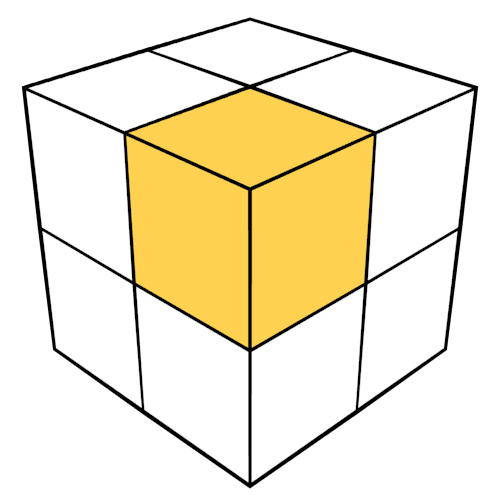
\includegraphics[width=0.19\textwidth]{./img/raw/octree/level_1.png}};
    \node[inner sep=0pt] (level_2) at (-8.25,-5cm)
         {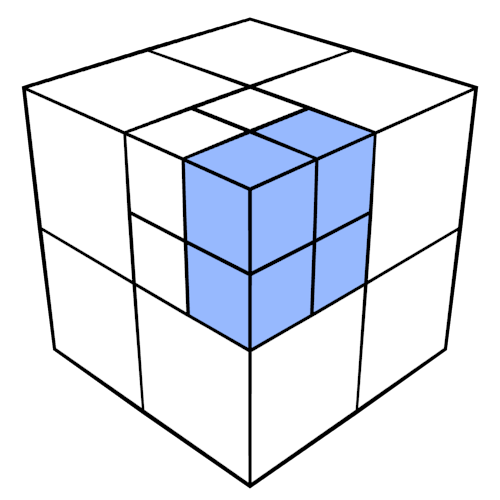
\includegraphics[width=0.19\textwidth]{./img/raw/octree/level_2.png}};

    % Text octree images
    \node (i1) at (-8.25, 1.75) {};
    \node (i2) at (-8.25, .25) {};
    \node (i3) at (-8.25, -2.25) {};
    \node (i4) at (-8.25, -3.75) {};

    % Arrows octree images
    \node (l1) at (-10.5,  3) {Laag $0$};
    \node (l1) at (-10.5, -1) {Laag $1$};
    \node (l1) at (-10.5, -5) {Laag $2$};

    \draw[-latex]  (i1) -> (i2);
    \draw[-latex]  (i3) -> (i4);

    % Legend
    \node[draw, rectangle, minimum width=0.5cm, minimum height=0.5cm, thick, fill=pastel_orange] (legend1) at (6.75, 3.98) {};
    \node[draw, rectangle, minimum width=0.5cm, minimum height=0.5cm, thick, fill=pastel_blue] (legend2) at (6.75, 3.38) {};
    \node[draw, rectangle, minimum width=0.5cm, minimum height=0.5cm, thick] (legend3) at (6.75, 2.78) {};

    \node[anchor=west] (legend1_text) at (7.1, 3.98) {Vertakkingsknoop};
    \node[anchor=west] (legend1_text) at (7.1, 3.38) {Volle bladknoop};
    \node[anchor=west] (legend1_text) at (7.1, 2.78) {Lege bladknoop};

    % Pointer representation octrees
    \node[circle,draw, minimum size=1cm, thick,fill=pastel_orange] (v1) at  (0,3cm) {};

    \node[circle,draw, minimum size=1cm, thick] (v11) at  (-5.25cm, -1cm) {};
    \node[circle,draw, minimum size=1cm, thick] (v12) at  (-3.75cm, -1cm) {};
    \node[circle,draw, minimum size=1cm,fill=pastel_orange, thick] (v13) at  (-2.25cm, -1cm) {};
    \node[circle,draw, minimum size=1cm, thick] (v14) at  (-0.75cm, -1cm) {};
    \node[circle,draw, minimum size=1cm, thick] (v15) at  (0.75cm, -1cm) {};
    \node[circle,draw, minimum size=1cm, thick] (v16) at  (2.25cm, -1cm) {};
    \node[circle,draw, minimum size=1cm, thick] (v17) at  (3.75cm, -1cm) {};
    \node[circle,draw, minimum size=1cm, thick] (v18) at  (5.25cm, -1cm) {};

    \node[circle,draw, minimum size=1cm, thick, fill=pastel_blue] (v21) at  (-5.25cm, -5cm) {};
    \node[circle,draw, minimum size=1cm, thick, fill=pastel_blue] (v22) at  (-3.75cm, -5cm) {};
    \node[circle,draw, minimum size=1cm, thick, fill=pastel_blue] (v23) at  (-2.25cm, -5cm) {};
    \node[circle,draw, minimum size=1cm, thick, fill=pastel_blue] (v24) at  (-0.75cm, -5cm) {};
    \node[circle,draw, minimum size=1cm, thick] (v25) at  (0.75cm, -5cm) {};
    \node[circle,draw, minimum size=1cm, thick] (v26) at  (2.25cm, -5cm) {};
    \node[circle,draw, minimum size=1cm, thick] (v27) at  (3.75cm, -5cm) {};
    \node[circle,draw, minimum size=1cm, thick] (v28) at  (5.25cm, -5cm) {};


    \draw[->] (v1) -- (v11);
    \draw[->] (v1) -- (v12);
    \draw[->] (v1) -- (v13);
    \draw[->] (v1) -- (v14);
    \draw[->] (v1) -- (v15);
    \draw[->] (v1) -- (v16);
    \draw[->] (v1) -- (v17);
    \draw[->] (v1) -- (v18);

    \draw[->] (v13) -- (v21);
    \draw[->] (v13) -- (v22);
    \draw[->] (v13) -- (v23);
    \draw[->] (v13) -- (v24);
    \draw[->] (v13) -- (v25);
    \draw[->] (v13) -- (v26);
    \draw[->] (v13) -- (v27);
    \draw[->] (v13) -- (v28);
  \end{tikzpicture}
  }

  \caption{Weergave van een octree bestaande uit drie lagen, links is de 3d representatie weergegeven, rechts de pointerrepresentatie .}
  \label{fig:hs-octree}
\end{figure}
